\chapter{如何知道训练有效：从损失到完整任务}
\section{训练损失正在下降，究竟学到了什么}
训练目标是让目标JSON中的token获得更高概率。开始时，模型可能在字段名称、格式、中文回复、动作名称或时长上与示范不同。只要这些差异减少，损失就可能下降。因此，损失下降是学习信号，但它把多种能力混合在一起，不能单凭一个数字判断踢球是否更准确。

例如，“回复更接近示范措辞”“更稳定输出五个字段”“选对了踢球脚”都会改变损失。前两项改善可能很快，第三项仍需要基于任务的独立检查。相邻步损失也会因抽到的四条样本难度不同而上下波动，不能把某一步低损失当成所有场景都已经学会。

\begin{figure}[htbp]
\centering
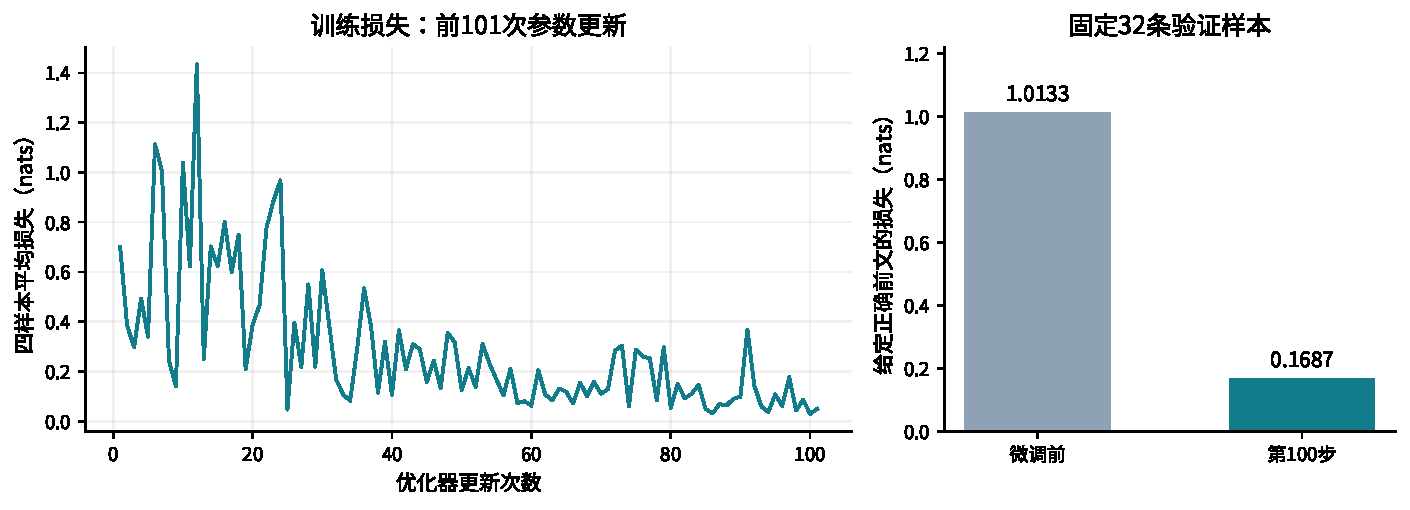
\includegraphics[width=\linewidth]{assets/training_snapshot.pdf}
\caption{真实日志快照：前101步训练损失，以及固定32条验证样本的teacher-forced损失。两个面板对应不同数据，不能直接互换解释；本图不包含微调后闭环成功率。}
\end{figure}

本书冻结的快照显示：训练前，32条固定验证样本的平均损失为1.013274；第100次更新时为0.168665。图中的nats表示使用自然对数计算的损失单位。这个下降说明模型更倾向于输出这些已知验证示范中的目标token。验证集没有参与反向更新，但反复查看同一小子集仍可能影响选模，最终必须在独立任务上验证。

\section{第一级：代码、数值与数据一致性}
首先检查程序有没有正确训练：输入长度是否超限；图片是否与样本对应；模型是否只更新指定参数；梯度是否有限；优化器步数与数据游标是否一致；保存和恢复后是否从正确位置继续；数据文件和基础模型的哈希是否符合固定清单。

当前流程已经做过短训练资源验证、恢复检查，以及正式第10步适配器与优化器状态核验。LoRA-B参数出现实际非零更新，说明训练不是只打印日志。它仍属于实现与资源证据，不是学习效果验收。

\section{第二级：给定画面时，模型自己生成什么}
训练期间的teacher forcing会给模型提供此前的正确目标token；真正生成时，后续内容依赖模型自己刚生成的token。一次早期格式错误可能影响整个JSON，所以必须单独做无强制答案的生成测试。

当前 \texttt{predict\_examples()} 会删除输入中的助手目标，只保留生成起点之前的内容，采用贪心生成，最多生成192个新token，然后把原始输出交给同一严格JSON解析器。原始输出和解析错误都写入 \texttt{predictions.jsonl}，没有偷偷修正成正确动作。

\begin{longtable}{P{33mm}P{58mm}P{60mm}}
\toprule
指标 & 当前定义 & 解释边界\\
\midrule
\endhead
JSON合法率 & 被严格解析器完整接受的输出数 / 全部样本数 & 仅合法不代表动作合适\\
type准确率 & action type与目标一致的样本数 / 全部样本数 & 区分skill、answer、clarify、finish\\
skill准确率 & skill字段与目标一致 / 全部样本数 & 包括非动作样本中null的匹配，不等于纯动作分类准确率\\
颜色准确率 & target\_color字段完全匹配 / 全部样本数 & 无颜色任务的null也计入\\
时长准确率 & seconds字段数值完全匹配 / 全部样本数 & 合理但不同的时长仍可能算错\\
联合准确率 & 上面四个字段同时匹配 / 全部样本数 & 不校验reply语义，不代表物理成功\\
分类型统计 & 每个skill或回复类型的样本数、合法数、联合正确数 & 目前小子集每类样本很少，波动较大\\
\bottomrule
\end{longtable}

解析失败样本在准确率分母中保留，并记为不正确。这样可以避免“只看解析成功的那部分”人为抬高准确率。另一方面，\texttt{reply}的描述是否忠实于图像，仍需要单独评价；不能因为四个结构字段一致就认为自由问答完全正确。

\section{当前确实存在的基线结果}
固定24条分层验证样本在未微调基础模型上的结果如下。该小集合按技能与回复类型抽样，用来作快速对照，并不是全量验证集的比例估计。

\begin{center}
\begin{tabular}{lr}
\toprule
未微调基线指标 & 结果\\
\midrule
JSON合法率 & 20/24 = 83.3\%\\
type准确率 & 75.0\%\\
skill准确率（含null） & 29.2\%\\
颜色准确率（含null） & 70.8\%\\
时长准确率 & 37.5\%\\
四字段联合准确率 & 6/24 = 25.0\%\\
\bottomrule
\end{tabular}
\end{center}

截至本书快照，正式训练后尚未完成这一组生成指标与闭环测试。早期资源试跑使用过不同版本提示词，其结果不能混入这次v5正式实验。第100步的验证损失改善也不能替代尚未完成的生成测试。

\section{第三级：在仿真中从头完成任务}
离线评测给模型的是规则老师轨迹上的观测。部署时，模型自己的选择会改变下一幅画面：少走一点、多转一点、提前踢一下，都会产生训练中较少见的状态。这种输入分布变化，是行为克隆需要闭环验证的主要原因。

完整踢球验收应从新的初始状态开始，给出明确颜色指令，允许模型搜索、靠近、对齐、踢球，最后由独立程序读取真实接触和位移证据。需要同时报告：
\begin{enumerate}
\item 目标是否找到，是否在看不到目标时错误声称目标不存在。
\item 是否到达可踢位置，是否重复动作、来回振荡或过早结束。
\item 是否选择正确颜色、正确脚，是否碰到非目标球。
\item 踢前是否提前推球，踢球是否产生目标脚接触与足够位移。
\item 是否恢复站稳，有无摔倒、超时、拒绝或决策次数耗尽。
\item 总模型调用次数、每次推理耗时、总墙钟时间和仿真时间。
\end{enumerate}

近脚已对准任务和随机远距离任务必须分开。前者只需较少动作，后者包含搜索和长期控制。把两类混合后得到较高成功率，可能掩盖导航能力不足。

当前默认VLM上限是40次决策；采集的合格踢球示范中，有40个任务需要超过40次决策，最长117次。因此后续闭环对照应显式设为 \texttt{--vlm-max-steps 120}，并独立记录每任务600秒墙钟上限。调整上限只保证任务有足够机会执行，不保证它会成功。

\section{怎样公平比较QLoRA与“方案一”}
\begin{enumerate}
\item 保持训练、验证、测试种子划分相同，按验证集选择设置，最后才使用测试集报告成绩。
\item 两种模型获得相同两路图像、语言、姿态、RGB-D辅助测量与历史长度。若一方没有深度辅助，应单独列为另一实验。
\item 保持相同技能库、执行器恢复时间、guard条件、每任务决策和墙钟上限。
\item 分别统计九个技能、三种颜色、盲区搜索、近脚踢球和直接运动，而不只看总体平均。
\item 报告显存、首轮特征提取成本、训练时间、在线决策延迟和成功率。冻结头缓存后的训练速度不能直接当成整套部署速度。
\item 从原始预训练VLM提特征的方案，与从QLoRA适配后的VLM提特征的方案应分开命名；后者已经利用了前一轮训练。
\end{enumerate}

\section{失败数据什么时候能够帮助学习}
当前保留了23个失败踢球任务的原始记录，但没有把它们作为正确动作监督。仅保存“失败了”的标签，不会自动告诉模型哪一步应该改成什么动作。

下一轮有三种不同处理方式。第一种是人工或可靠老师为失败状态补上正确的下一步动作，形成新的SFT样本；第二种是构造同一输入下经过核验的较好和较差输出，用于偏好学习；第三种是在可控仿真中定义奖励并训练策略。三者需要不同数据与训练目标，不能把失败轨迹直接混入当前成功示范JSON损失中。

对于这个项目，补充模型实际走偏后的状态尤其有价值。比如“红球仍在左侧，刚才右转错误，下一步应当左转纠正”需要真实观测、允许的执行历史和经过验证的纠正动作。纠正动作不能只根据最终失败倒推猜测，也不应把后续才知道的真实结果放回当前输入。

\section{完成这一轮之后，怎样决定下一步}
先检查生成输出是否稳定合法、运动命令是否能执行一次后结束，再评估近脚踢球，最后评估盲区搜索与随机远距离踢球。如果格式很好而搜索差，优先检查搜索数据与历史表示；如果目标颜色常错，检查同一画面不同语言目标的数据覆盖；如果对齐时来回摆动，检查距离特征、动作时长分布及规则老师隐藏锁脚状态。

还应单独检查视野问答。当前监督主要描述球，不应把模型答出某些新物体名称视为已验证能力。开放问答需要新的场景、多样物体及明确评价准则。模型训练完成这个文件状态，只表示优化流程到达计划终点；是否适合接入日常交互，要由这些具体评测决定。
